\section{Diskussion}
\label{sec:Diskussion}

Zunächst wird das experimentell bestimmte Verhältnis 
\begin{align*}
\bigl(\frac{\mathrm{h}}{\mathrm{e_0}}\bigr)_\text{exp} = (3,58 \pm 0,23)\cdot 10^{-15}\,\si{\eV\second} 
\end{align*}
mit dem Literaturwert 
\begin{align*}
\bigl(\frac{\mathrm{h}}{\mathrm{e_0}}\bigr)_\text{Literatur} = 4,14 \cdot 10^{-15}\,\si{\eV\second}, 
\end{align*}
mit $\mathrm{h} = \SI{6.626070040e-34}{\joule\second}$ \cite{h} und $\mathrm{e_0} = \SI{1.6021766208e-19}{\coulomb}$ \cite{e} verglichen.
Hierbei ergibt sich eine relative Abweichung von $13,53\%$, welche verhältnismäßig klein ist.
Diese lässt sich durch den empfindlichen Versuchsaufbau sowie einen zwischenzeitlich vorhandenen
Wackelkontakt der Photozelle und andere Lichtquellen erklären.

\noindent Bei Betrachtung der Abbildung \ref{fig:gelb2} fallen einige Besonderheiten auf.
Die Kurve erreicht entsprechend der Theorie bei hoher Beschleunigungsspannung einen Sättiungswert,
da alle ausgelösten Elektronen die Anode erreichen. Hierbei ist die Anzahl der ausgelösten Elektronen
nicht mehr von der Beschleunigungsspannung, sondern ausschließlich von der Lichtintensität abhängig.
Es ist weiter zu erkennen, dass der Photostrom bereits vor Erreichen der Grenzspannung $U_\text{G}$
beginnt zu sinken, was sich durch die Fermi-Dirac-Verteilung erklären lässt. Nach dieser besitzen die
Elektronen schon vor der Bestrahlung mit Licht unterschiedliche kinetische Energien, sodass viele
schon vor der Grenzspannung nicht mehr die Anode erreichen können. Zusätzlich kann, da das 
Kathodenmaterial bei einer Temperatur von $\SI{20}{\celsius}$
verdampft \cite{kent}, ein entgegengesetzter Strom auftreten, 
der die thermische Elektronenemission begünstigt, die dem Photostrom entgegenwirkt.

\section{Anhang}
\label{Anhang}
Im folgenden sind die Kopien der Messwerte aufgelistet.

\begin{figure}[H]
  \centering
  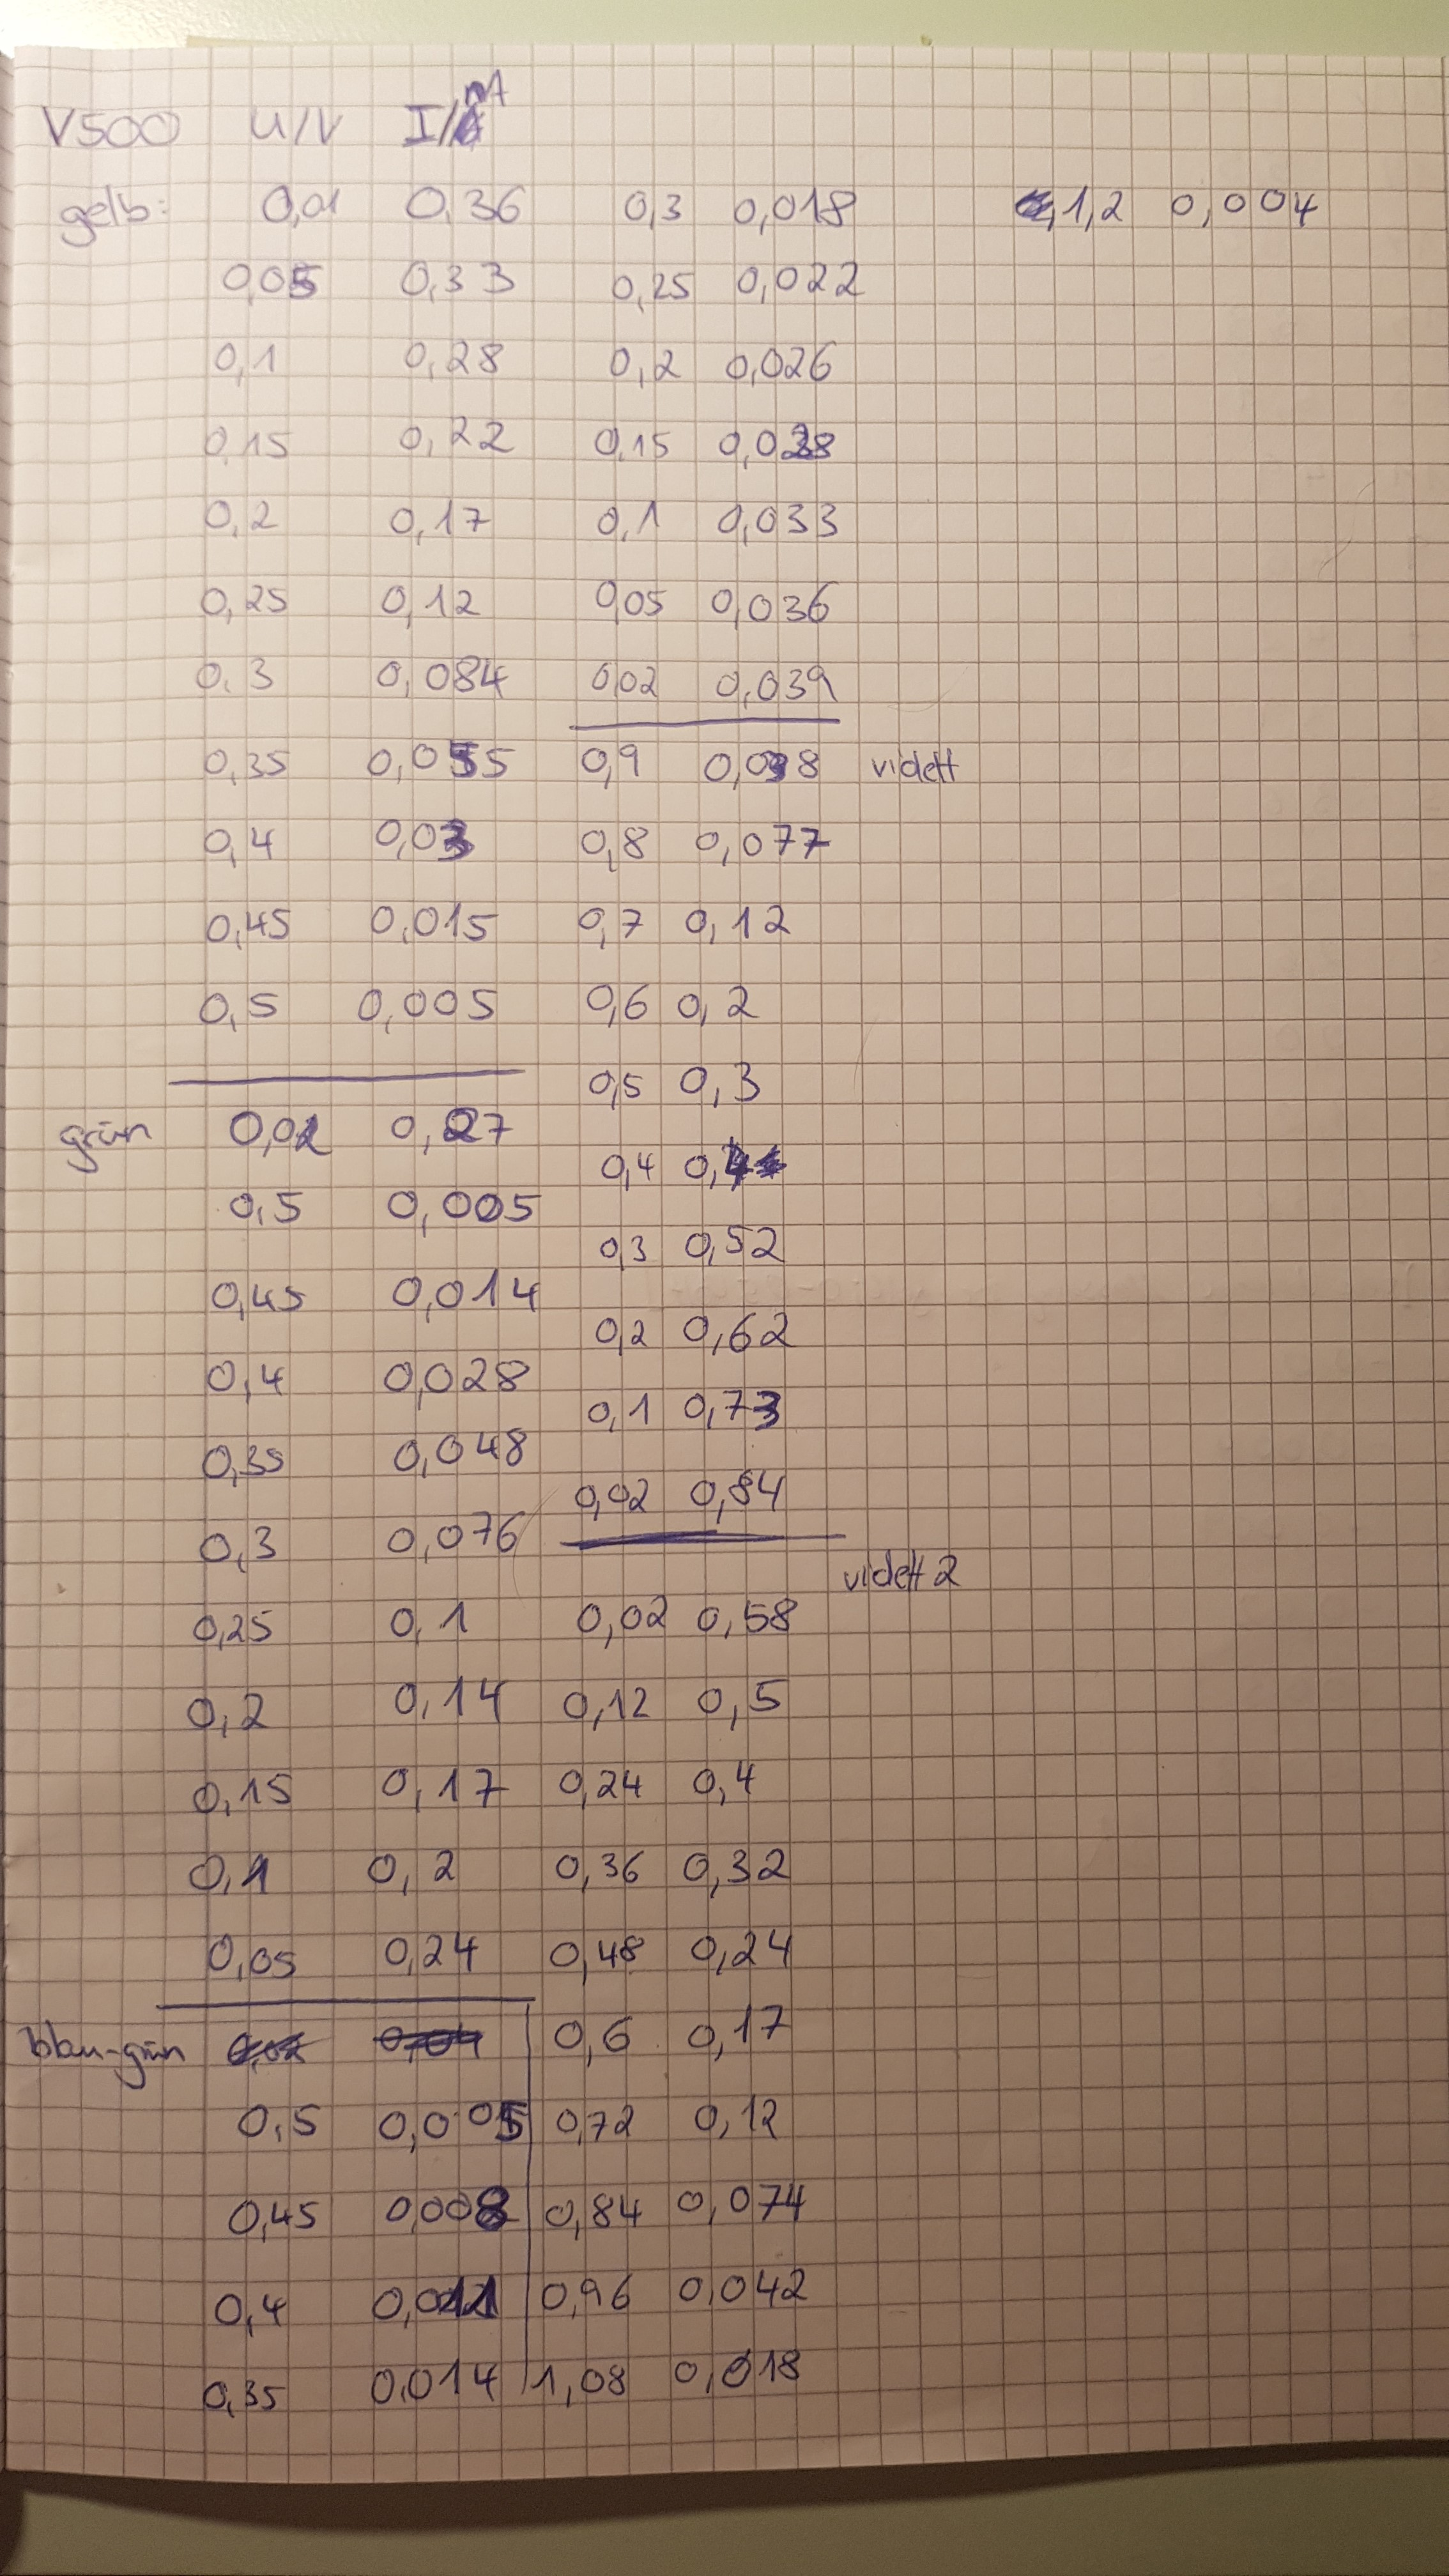
\includegraphics[height=24cm]{1.jpg}
\end{figure}

\begin{figure}[H]
  \centering
  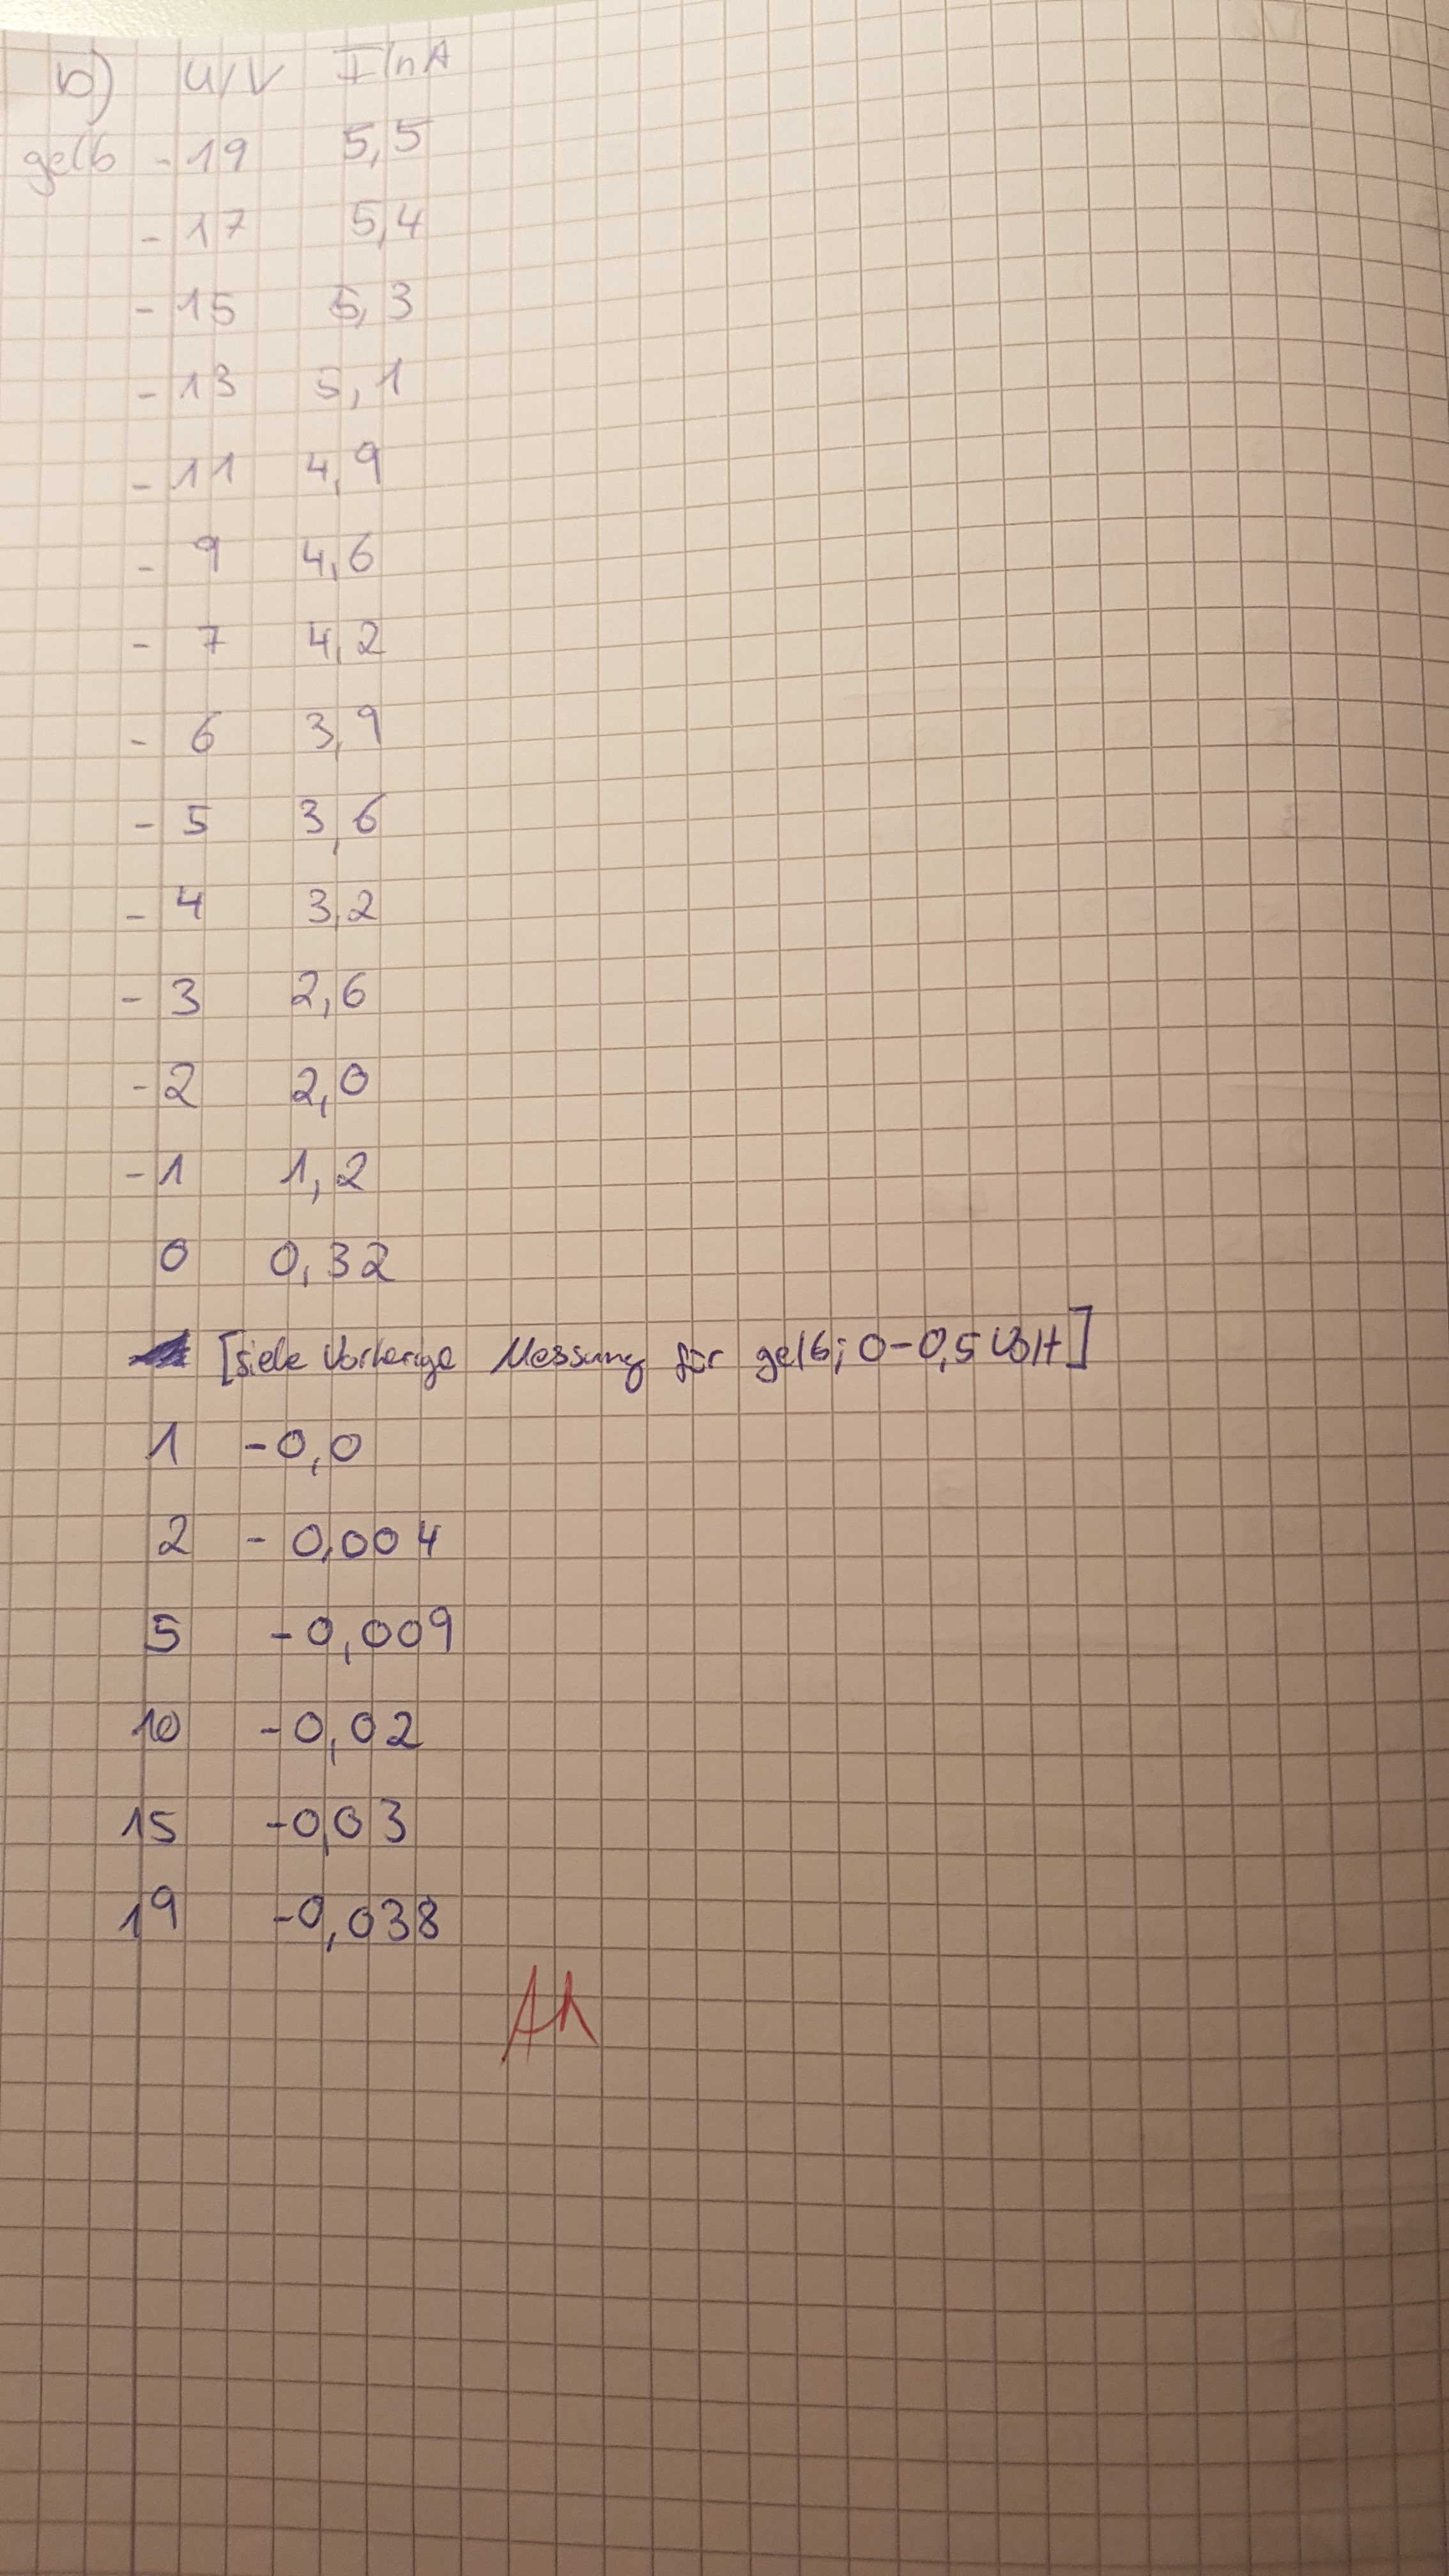
\includegraphics[height=24cm]{2.jpg}
\end{figure}

